\chapter{Lab Assignments}

In these labs you can use any programming language that you want. 
In each assignment you must deliver the source code and a brief explanatory document explaining how you solved the assignment.
It should also include some examples, including the commands that you used to test it and the results.
Some assignments may ask for additional information, such as plots.

Pack all the files in a zip file (not rar) and submit it using moodle.
Remember to include the names and NIA in all the source files and in the document.

Prepare the assignment in advance, so that you can complete it during the class.
The submission deadline will be one week after the class.

\section{Traffic Generator and Sink}

In this lab assignment you will program a Poisson traffic generator and a traffic sink.
The Poisson traffic generator takes the following parameters:
destination host, destination port, packet rate and traffic class.

It generates UDP packets with a string that contains three integer values separated by a blank space. The integers represents a packet id (starting with 0), time stamp in milliseconds (local significance only) and traffic class.

The traffic sink takes a port number as a parameter and computes packet delay and packet loss for each packet class (computation of jitter is optional).

Test it with a traffic generation rate of 10 packets per second.

Note that since the generator and the sink are directly connected, the delay, the jitter and the packet loss will will be zero.

In the next assignment we will place a queue in between and these values will no longer be zero.

\section{A queue}

The second module that you have to construct in this course contains a queue (that includes a dropper a buffer) and a scheduler.

Note that each module has to be a separate program. The different modules communicate (send packets to each other) using sockets.

This program listens at an udp port and transmits the packets to a given udp port and address. Consequently, it has to be simultaneously an UDP server and an UDP client. You may consider the possibility of using different threads for the dropper and the scheduler.

All port numbers and the destination should be configurable as parameters. An additional parameter will configure the queue size (number of packets). If the queue size is set to zero, it means infinite queue length. If a finite queue is used, a taildrop policy will be applied.

The scheduler should be configurable to be able to choose an exponentially distributed service time or a deterministic service time. In either case, the service rate should be taken as an input parameter.

Combine the Buffer with the traffic generator and traffic sink modules to make measures of packet loss and delay.

\begin{figure}[!h]
\centering
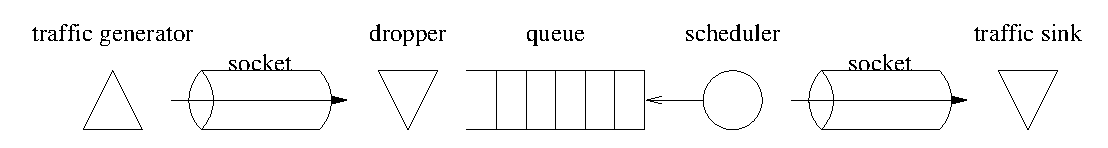
\includegraphics[width=\linewidth]{figures/scenario.eps}
\caption{Scenario to test in lab assignment 2.}
\label{fig:scenario}
\end{figure}

